% !TEX TS-program = pdflatex
% !TEX encoding = UTF-8 Unicode
\documentclass[border=0mm]{standalone}
% packages
\usepackage{tikz}
\usetikzlibrary{patterns}
\usepackage{amsmath,amssymb}
\usepackage{bm}
\usepackage{pgfplots}
\pgfplotsset{compat=1.15}
% start document
\begin{document}
% generated by ROOT (CERN)
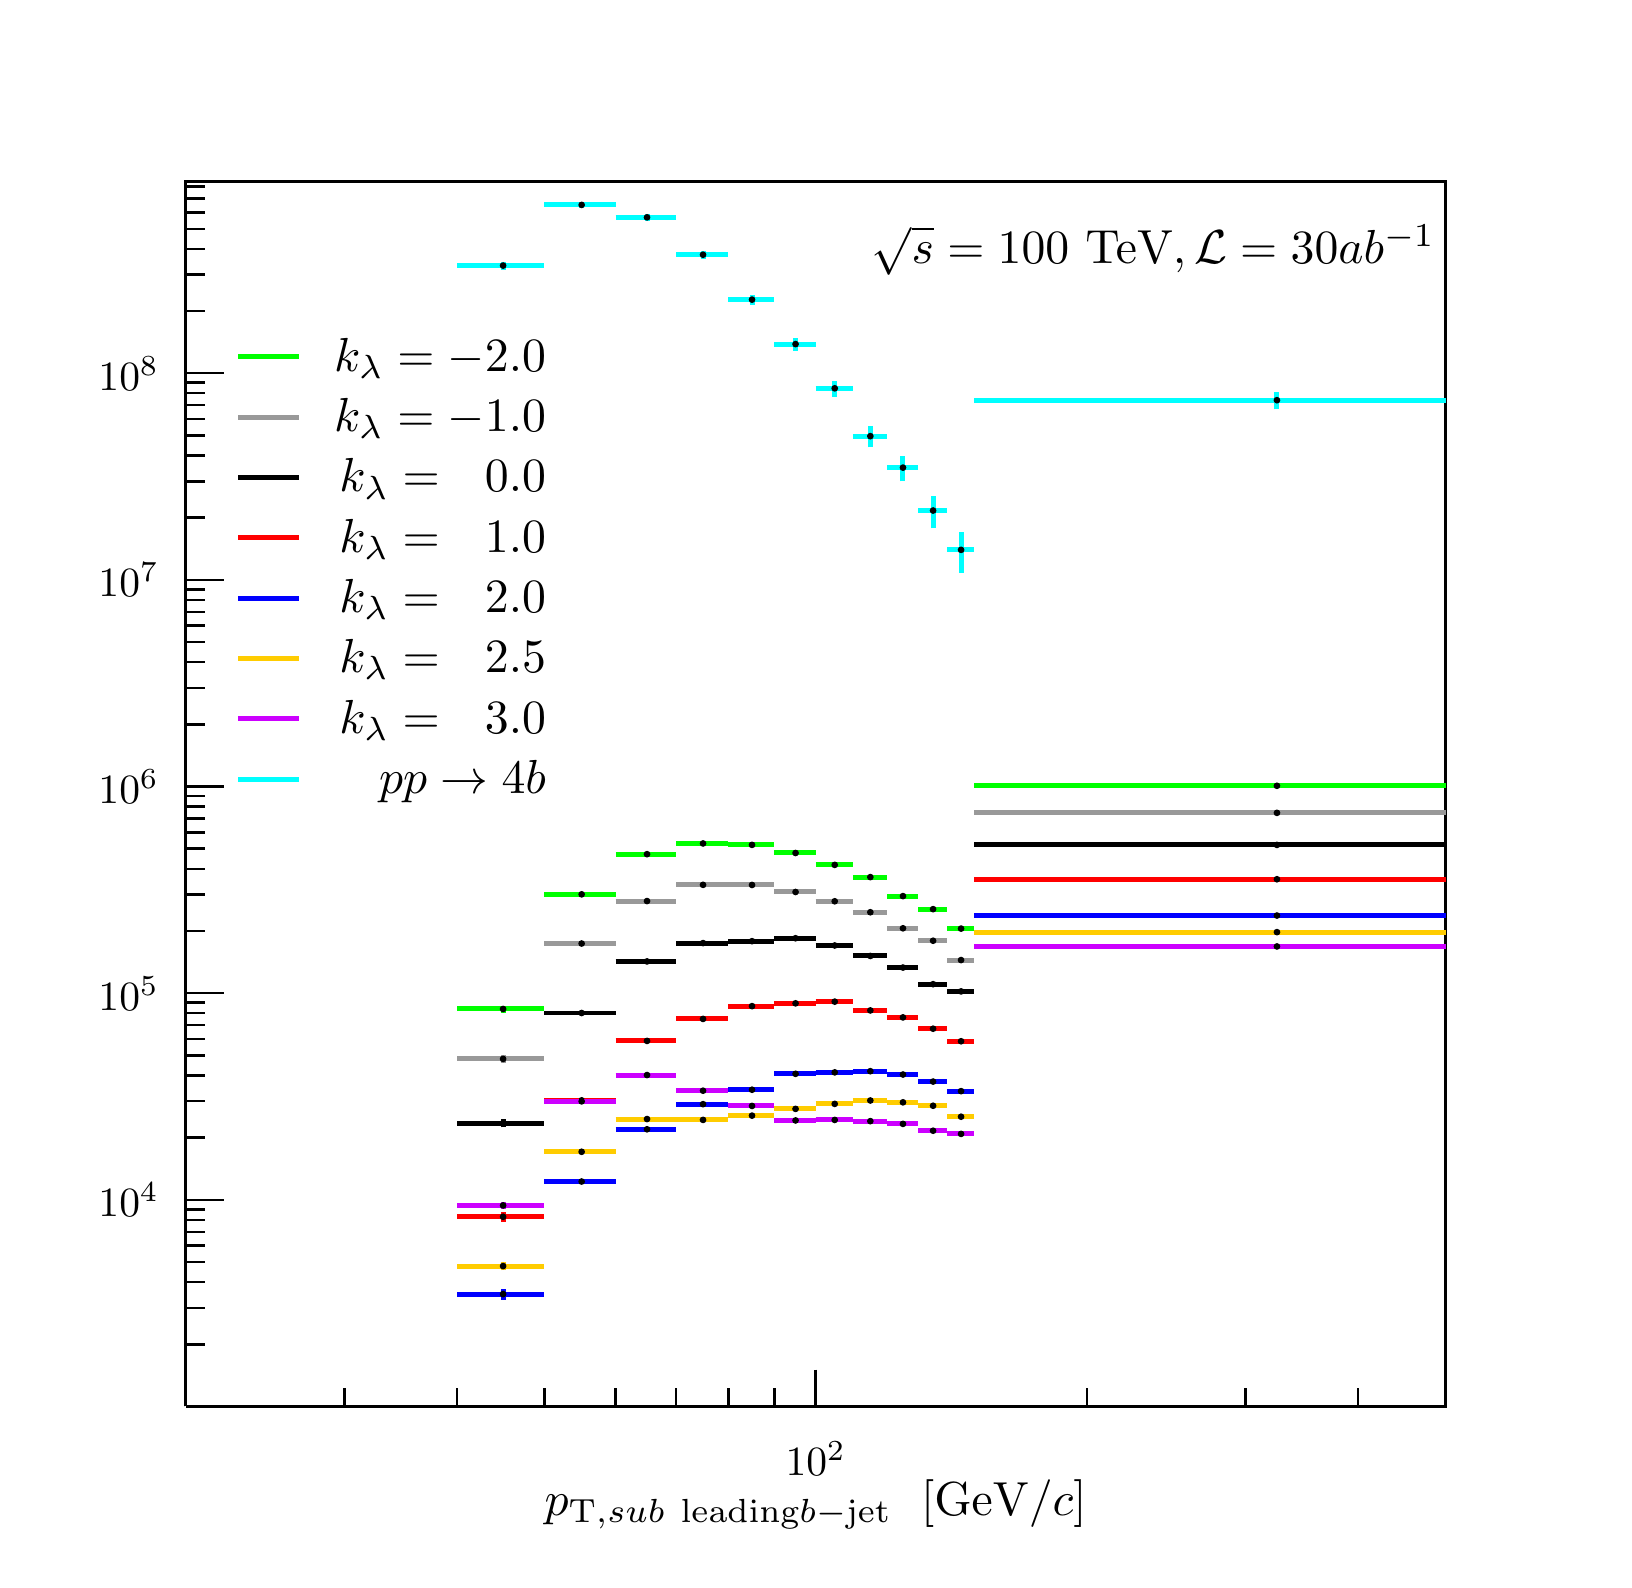
\begin{tikzpicture}
\pgfdeclareplotmark{cross} {
\pgfpathmoveto{\pgfpoint{-0.3\pgfplotmarksize}{\pgfplotmarksize}}
\pgfpathlineto{\pgfpoint{+0.3\pgfplotmarksize}{\pgfplotmarksize}}
\pgfpathlineto{\pgfpoint{+0.3\pgfplotmarksize}{0.3\pgfplotmarksize}}
\pgfpathlineto{\pgfpoint{+1\pgfplotmarksize}{0.3\pgfplotmarksize}}
\pgfpathlineto{\pgfpoint{+1\pgfplotmarksize}{-0.3\pgfplotmarksize}}
\pgfpathlineto{\pgfpoint{+0.3\pgfplotmarksize}{-0.3\pgfplotmarksize}}
\pgfpathlineto{\pgfpoint{+0.3\pgfplotmarksize}{-1.\pgfplotmarksize}}
\pgfpathlineto{\pgfpoint{-0.3\pgfplotmarksize}{-1.\pgfplotmarksize}}
\pgfpathlineto{\pgfpoint{-0.3\pgfplotmarksize}{-0.3\pgfplotmarksize}}
\pgfpathlineto{\pgfpoint{-1.\pgfplotmarksize}{-0.3\pgfplotmarksize}}
\pgfpathlineto{\pgfpoint{-1.\pgfplotmarksize}{0.3\pgfplotmarksize}}
\pgfpathlineto{\pgfpoint{-0.3\pgfplotmarksize}{0.3\pgfplotmarksize}}
\pgfpathclose
\pgfusepathqstroke
}
\pgfdeclareplotmark{cross*} {
\pgfpathmoveto{\pgfpoint{-0.3\pgfplotmarksize}{\pgfplotmarksize}}
\pgfpathlineto{\pgfpoint{+0.3\pgfplotmarksize}{\pgfplotmarksize}}
\pgfpathlineto{\pgfpoint{+0.3\pgfplotmarksize}{0.3\pgfplotmarksize}}
\pgfpathlineto{\pgfpoint{+1\pgfplotmarksize}{0.3\pgfplotmarksize}}
\pgfpathlineto{\pgfpoint{+1\pgfplotmarksize}{-0.3\pgfplotmarksize}}
\pgfpathlineto{\pgfpoint{+0.3\pgfplotmarksize}{-0.3\pgfplotmarksize}}
\pgfpathlineto{\pgfpoint{+0.3\pgfplotmarksize}{-1.\pgfplotmarksize}}
\pgfpathlineto{\pgfpoint{-0.3\pgfplotmarksize}{-1.\pgfplotmarksize}}
\pgfpathlineto{\pgfpoint{-0.3\pgfplotmarksize}{-0.3\pgfplotmarksize}}
\pgfpathlineto{\pgfpoint{-1.\pgfplotmarksize}{-0.3\pgfplotmarksize}}
\pgfpathlineto{\pgfpoint{-1.\pgfplotmarksize}{0.3\pgfplotmarksize}}
\pgfpathlineto{\pgfpoint{-0.3\pgfplotmarksize}{0.3\pgfplotmarksize}}
\pgfpathclose
\pgfusepathqfillstroke
}
\pgfdeclareplotmark{newstar} {
\pgfpathmoveto{\pgfqpoint{0pt}{\pgfplotmarksize}}
\pgfpathlineto{\pgfqpointpolar{44}{0.5\pgfplotmarksize}}
\pgfpathlineto{\pgfqpointpolar{18}{\pgfplotmarksize}}
\pgfpathlineto{\pgfqpointpolar{-20}{0.5\pgfplotmarksize}}
\pgfpathlineto{\pgfqpointpolar{-54}{\pgfplotmarksize}}
\pgfpathlineto{\pgfqpointpolar{-90}{0.5\pgfplotmarksize}}
\pgfpathlineto{\pgfqpointpolar{234}{\pgfplotmarksize}}
\pgfpathlineto{\pgfqpointpolar{198}{0.5\pgfplotmarksize}}
\pgfpathlineto{\pgfqpointpolar{162}{\pgfplotmarksize}}
\pgfpathlineto{\pgfqpointpolar{134}{0.5\pgfplotmarksize}}
\pgfpathclose
\pgfusepathqstroke
}
\pgfdeclareplotmark{newstar*} {
\pgfpathmoveto{\pgfqpoint{0pt}{\pgfplotmarksize}}
\pgfpathlineto{\pgfqpointpolar{44}{0.5\pgfplotmarksize}}
\pgfpathlineto{\pgfqpointpolar{18}{\pgfplotmarksize}}
\pgfpathlineto{\pgfqpointpolar{-20}{0.5\pgfplotmarksize}}
\pgfpathlineto{\pgfqpointpolar{-54}{\pgfplotmarksize}}
\pgfpathlineto{\pgfqpointpolar{-90}{0.5\pgfplotmarksize}}
\pgfpathlineto{\pgfqpointpolar{234}{\pgfplotmarksize}}
\pgfpathlineto{\pgfqpointpolar{198}{0.5\pgfplotmarksize}}
\pgfpathlineto{\pgfqpointpolar{162}{\pgfplotmarksize}}
\pgfpathlineto{\pgfqpointpolar{134}{0.5\pgfplotmarksize}}
\pgfpathclose
\pgfusepathqfillstroke
}
\definecolor{c}{rgb}{1,1,1};
\draw [color=c, fill=c] (0,0) rectangle (20,19.4486);
\draw [color=c, fill=c] (0,0) rectangle (20,19.4486);
\draw [color=c, fill=c] (2,1.94486) rectangle (18,17.5038);
\definecolor{c}{rgb}{0,0,0};
\draw [c,line width=0.9] (2,1.94486) -- (2,17.5038) -- (18,17.5038) -- (18,1.94486) -- (2,1.94486);
\definecolor{c}{rgb}{1,1,1};
\draw [color=c, fill=c] (2,1.94486) rectangle (18,17.5038);
\definecolor{c}{rgb}{0,0,0};
\draw [c,line width=0.9] (2,1.94486) -- (2,17.5038) -- (18,17.5038) -- (18,1.94486) -- (2,1.94486);
\definecolor{c}{rgb}{0,1,1};
\draw [c,line width=1.8] (6.03087,16.3805) -- (6.03087,16.434);
\draw [c,line width=1.8] (6.03087,16.434) -- (6.03087,16.4852);
\draw [c,line width=1.8] (5.44541,16.434) -- (6.03087,16.434);
\draw [c,line width=1.8] (6.03087,16.434) -- (6.55459,16.434);
\definecolor{c}{rgb}{0,0,0};
\foreach \P in {(6.03087,16.434)}{\draw[mark options={color=c,fill=c},mark size=2.402402pt,mark=*,mark size=1pt] plot coordinates {\P};}
\definecolor{c}{rgb}{0,1,1};
\draw [c,line width=1.8] (7.02834,17.1668) -- (7.02834,17.2047);
\draw [c,line width=1.8] (7.02834,17.2047) -- (7.02834,17.2414);
\draw [c,line width=1.8] (6.55459,17.2047) -- (7.02834,17.2047);
\draw [c,line width=1.8] (7.02834,17.2047) -- (7.46085,17.2047);
\definecolor{c}{rgb}{0,0,0};
\foreach \P in {(7.02834,17.2047)}{\draw[mark options={color=c,fill=c},mark size=2.402402pt,mark=*,mark size=1pt] plot coordinates {\P};}
\definecolor{c}{rgb}{0,1,1};
\draw [c,line width=1.8] (7.85872,17.0059) -- (7.85872,17.0466);
\draw [c,line width=1.8] (7.85872,17.0466) -- (7.85872,17.0859);
\draw [c,line width=1.8] (7.46085,17.0466) -- (7.85872,17.0466);
\draw [c,line width=1.8] (7.85872,17.0466) -- (8.22708,17.0466);
\definecolor{c}{rgb}{0,0,0};
\foreach \P in {(7.85872,17.0466)}{\draw[mark options={color=c,fill=c},mark size=2.402402pt,mark=*,mark size=1pt] plot coordinates {\P};}
\definecolor{c}{rgb}{0,1,1};
\draw [c,line width=1.8] (8.57002,16.5214) -- (8.57002,16.5718);
\draw [c,line width=1.8] (8.57002,16.5718) -- (8.57002,16.6199);
\draw [c,line width=1.8] (8.22708,16.5718) -- (8.57002,16.5718);
\draw [c,line width=1.8] (8.57002,16.5718) -- (8.89083,16.5718);
\definecolor{c}{rgb}{0,0,0};
\foreach \P in {(8.57002,16.5718)}{\draw[mark options={color=c,fill=c},mark size=2.402402pt,mark=*,mark size=1pt] plot coordinates {\P};}
\definecolor{c}{rgb}{0,1,1};
\draw [c,line width=1.8] (9.19217,15.9365) -- (9.19217,16.0015);
\draw [c,line width=1.8] (9.19217,16.0015) -- (9.19217,16.063);
\draw [c,line width=1.8] (8.89083,16.0015) -- (9.19217,16.0015);
\draw [c,line width=1.8] (9.19217,16.0015) -- (9.47629,16.0015);
\definecolor{c}{rgb}{0,0,0};
\foreach \P in {(9.19217,16.0015)}{\draw[mark options={color=c,fill=c},mark size=2.402402pt,mark=*,mark size=1pt] plot coordinates {\P};}
\definecolor{c}{rgb}{0,1,1};
\draw [c,line width=1.8] (9.74504,15.3527) -- (9.74504,15.4367);
\draw [c,line width=1.8] (9.74504,15.4367) -- (9.74504,15.5149);
\draw [c,line width=1.8] (9.47629,15.4367) -- (9.74504,15.4367);
\draw [c,line width=1.8] (9.74504,15.4367) -- (10,15.4367);
\definecolor{c}{rgb}{0,0,0};
\foreach \P in {(9.74504,15.4367)}{\draw[mark options={color=c,fill=c},mark size=2.402402pt,mark=*,mark size=1pt] plot coordinates {\P};}
\definecolor{c}{rgb}{0,1,1};
\draw [c,line width=1.8] (10.2425,14.7667) -- (10.2425,14.8754);
\draw [c,line width=1.8] (10.2425,14.8754) -- (10.2425,14.9745);
\draw [c,line width=1.8] (10,14.8754) -- (10.2425,14.8754);
\draw [c,line width=1.8] (10.2425,14.8754) -- (10.4738,14.8754);
\definecolor{c}{rgb}{0,0,0};
\foreach \P in {(10.2425,14.8754)}{\draw[mark options={color=c,fill=c},mark size=2.402402pt,mark=*,mark size=1pt] plot coordinates {\P};}
\definecolor{c}{rgb}{0,1,1};
\draw [c,line width=1.8] (10.6947,14.1237) -- (10.6947,14.2677);
\draw [c,line width=1.8] (10.6947,14.2677) -- (10.6947,14.3956);
\draw [c,line width=1.8] (10.4738,14.2677) -- (10.6947,14.2677);
\draw [c,line width=1.8] (10.6947,14.2677) -- (10.9063,14.2677);
\definecolor{c}{rgb}{0,0,0};
\foreach \P in {(10.6947,14.2677)}{\draw[mark options={color=c,fill=c},mark size=2.402402pt,mark=*,mark size=1pt] plot coordinates {\P};}
\definecolor{c}{rgb}{0,1,1};
\draw [c,line width=1.8] (11.1092,13.6943) -- (11.1092,13.8681);
\draw [c,line width=1.8] (11.1092,13.8681) -- (11.1092,14.0188);
\draw [c,line width=1.8] (10.9063,13.8681) -- (11.1092,13.8681);
\draw [c,line width=1.8] (11.1092,13.8681) -- (11.3041,13.8681);
\definecolor{c}{rgb}{0,0,0};
\foreach \P in {(11.1092,13.8681)}{\draw[mark options={color=c,fill=c},mark size=2.402402pt,mark=*,mark size=1pt] plot coordinates {\P};}
\definecolor{c}{rgb}{0,1,1};
\draw [c,line width=1.8] (11.4917,13.0976) -- (11.4917,13.3232);
\draw [c,line width=1.8] (11.4917,13.3232) -- (11.4917,13.5115);
\draw [c,line width=1.8] (11.3041,13.3232) -- (11.4917,13.3232);
\draw [c,line width=1.8] (11.4917,13.3232) -- (11.6725,13.3232);
\definecolor{c}{rgb}{0,0,0};
\foreach \P in {(11.4917,13.3232)}{\draw[mark options={color=c,fill=c},mark size=2.402402pt,mark=*,mark size=1pt] plot coordinates {\P};}
\definecolor{c}{rgb}{0,1,1};
\draw [c,line width=1.8] (11.8469,12.5352) -- (11.8469,12.8237);
\draw [c,line width=1.8] (11.8469,12.8237) -- (11.8469,13.0537);
\draw [c,line width=1.8] (11.6725,12.8237) -- (11.8469,12.8237);
\draw [c,line width=1.8] (11.8469,12.8237) -- (12.0154,12.8237);
\definecolor{c}{rgb}{0,0,0};
\foreach \P in {(11.8469,12.8237)}{\draw[mark options={color=c,fill=c},mark size=2.402402pt,mark=*,mark size=1pt] plot coordinates {\P};}
\definecolor{c}{rgb}{0,1,1};
\draw [c,line width=1.8] (15.8587,14.6081) -- (15.8587,14.7245);
\draw [c,line width=1.8] (15.8587,14.7245) -- (15.8587,14.8302);
\draw [c,line width=1.8] (12.0154,14.7245) -- (15.8587,14.7245);
\draw [c,line width=1.8] (15.8587,14.7245) -- (18,14.7245);
\definecolor{c}{rgb}{0,0,0};
\foreach \P in {(15.8587,14.7245)}{\draw[mark options={color=c,fill=c},mark size=2.402402pt,mark=*,mark size=1pt] plot coordinates {\P};}
\draw [c,line width=0.9] (2,1.94486) -- (18,1.94486);
\draw [c,line width=0.9] (4.01543,2.17825) -- (4.01543,1.94486);
\draw [c,line width=0.9] (5.4454,2.17825) -- (5.4454,1.94486);
\draw [c,line width=0.9] (6.55458,2.17825) -- (6.55458,1.94486);
\draw [c,line width=0.9] (7.46084,2.17825) -- (7.46084,1.94486);
\draw [c,line width=0.9] (8.22708,2.17825) -- (8.22708,1.94486);
\draw [c,line width=0.9] (8.89082,2.17825) -- (8.89082,1.94486);
\draw [c,line width=0.9] (9.47628,2.17825) -- (9.47628,1.94486);
\draw [c,line width=0.9] (9.99999,2.41163) -- (9.99999,1.94486);
\draw [anchor=base] (9.99999,1.06481) node[scale=1.50291, color=c, rotate=0]{$10^{2}$};
\draw [c,line width=0.9] (13.4454,2.17825) -- (13.4454,1.94486);
\draw [c,line width=0.9] (15.4608,2.17825) -- (15.4608,1.94486);
\draw [c,line width=0.9] (16.8908,2.17825) -- (16.8908,1.94486);
\draw [c,line width=0.9] (18,2.17825) -- (18,1.94486);
\draw (10,0.700151) node[scale=1.72557, color=c, rotate=0]{$ p_{\text{T}, sub ~\text{leading} b-\text{jet~}} ~[\text{GeV}/c]$};
\draw [c,line width=0.9] (2,1.94486) -- (2,17.5038);
\draw [c,line width=0.9] (2.24,2.7349) -- (2,2.7349);
\draw [c,line width=0.9] (2.24,3.19704) -- (2,3.19704);
\draw [c,line width=0.9] (2.24,3.52493) -- (2,3.52493);
\draw [c,line width=0.9] (2.24,3.77927) -- (2,3.77927);
\draw [c,line width=0.9] (2.24,3.98708) -- (2,3.98708);
\draw [c,line width=0.9] (2.24,4.16277) -- (2,4.16277);
\draw [c,line width=0.9] (2.24,4.31497) -- (2,4.31497);
\draw [c,line width=0.9] (2.24,4.44922) -- (2,4.44922);
\draw [c,line width=0.9] (2.48,4.56931) -- (2,4.56931);
\draw [anchor= east] (1.844,4.56931) node[scale=1.50291, color=c, rotate=0]{$10^{4}$};
\draw [c,line width=0.9] (2.24,5.35934) -- (2,5.35934);
\draw [c,line width=0.9] (2.24,5.82149) -- (2,5.82149);
\draw [c,line width=0.9] (2.24,6.14938) -- (2,6.14938);
\draw [c,line width=0.9] (2.24,6.40372) -- (2,6.40372);
\draw [c,line width=0.9] (2.24,6.61152) -- (2,6.61152);
\draw [c,line width=0.9] (2.24,6.78722) -- (2,6.78722);
\draw [c,line width=0.9] (2.24,6.93942) -- (2,6.93942);
\draw [c,line width=0.9] (2.24,7.07366) -- (2,7.07366);
\draw [c,line width=0.9] (2.48,7.19375) -- (2,7.19375);
\draw [anchor= east] (1.844,7.19375) node[scale=1.50291, color=c, rotate=0]{$10^{5}$};
\draw [c,line width=0.9] (2.24,7.98379) -- (2,7.98379);
\draw [c,line width=0.9] (2.24,8.44593) -- (2,8.44593);
\draw [c,line width=0.9] (2.24,8.77383) -- (2,8.77383);
\draw [c,line width=0.9] (2.24,9.02816) -- (2,9.02816);
\draw [c,line width=0.9] (2.24,9.23597) -- (2,9.23597);
\draw [c,line width=0.9] (2.24,9.41167) -- (2,9.41167);
\draw [c,line width=0.9] (2.24,9.56386) -- (2,9.56386);
\draw [c,line width=0.9] (2.24,9.69811) -- (2,9.69811);
\draw [c,line width=0.9] (2.48,9.8182) -- (2,9.8182);
\draw [anchor= east] (1.844,9.8182) node[scale=1.50291, color=c, rotate=0]{$10^{6}$};
\draw [c,line width=0.9] (2.24,10.6082) -- (2,10.6082);
\draw [c,line width=0.9] (2.24,11.0704) -- (2,11.0704);
\draw [c,line width=0.9] (2.24,11.3983) -- (2,11.3983);
\draw [c,line width=0.9] (2.24,11.6526) -- (2,11.6526);
\draw [c,line width=0.9] (2.24,11.8604) -- (2,11.8604);
\draw [c,line width=0.9] (2.24,12.0361) -- (2,12.0361);
\draw [c,line width=0.9] (2.24,12.1883) -- (2,12.1883);
\draw [c,line width=0.9] (2.24,12.3226) -- (2,12.3226);
\draw [c,line width=0.9] (2.48,12.4426) -- (2,12.4426);
\draw [anchor= east] (1.844,12.4426) node[scale=1.50291, color=c, rotate=0]{$10^{7}$};
\draw [c,line width=0.9] (2.24,13.2327) -- (2,13.2327);
\draw [c,line width=0.9] (2.24,13.6948) -- (2,13.6948);
\draw [c,line width=0.9] (2.24,14.0227) -- (2,14.0227);
\draw [c,line width=0.9] (2.24,14.2771) -- (2,14.2771);
\draw [c,line width=0.9] (2.24,14.4849) -- (2,14.4849);
\draw [c,line width=0.9] (2.24,14.6606) -- (2,14.6606);
\draw [c,line width=0.9] (2.24,14.8128) -- (2,14.8128);
\draw [c,line width=0.9] (2.24,14.947) -- (2,14.947);
\draw [c,line width=0.9] (2.48,15.0671) -- (2,15.0671);
\draw [anchor= east] (1.844,15.0671) node[scale=1.50291, color=c, rotate=0]{$10^{8}$};
\draw [c,line width=0.9] (2.24,15.8571) -- (2,15.8571);
\draw [c,line width=0.9] (2.24,16.3193) -- (2,16.3193);
\draw [c,line width=0.9] (2.24,16.6472) -- (2,16.6472);
\draw [c,line width=0.9] (2.24,16.9015) -- (2,16.9015);
\draw [c,line width=0.9] (2.24,17.1093) -- (2,17.1093);
\draw [c,line width=0.9] (2.24,17.285) -- (2,17.285);
\draw [c,line width=0.9] (2.24,17.4372) -- (2,17.4372);
\definecolor{c}{rgb}{0,1,0};
\draw [c,line width=1.8] (6.03087,6.94812) -- (6.03087,6.99292);
\draw [c,line width=1.8] (6.03087,6.99292) -- (6.03087,7.03603);
\draw [c,line width=1.8] (5.44541,6.99292) -- (6.03087,6.99292);
\draw [c,line width=1.8] (6.03087,6.99292) -- (6.55459,6.99292);
\definecolor{c}{rgb}{0,0,0};
\foreach \P in {(6.03087,6.99292)}{\draw[mark options={color=c,fill=c},mark size=2.402402pt,mark=*,mark size=1pt] plot coordinates {\P};}
\definecolor{c}{rgb}{0,1,0};
\draw [c,line width=1.8] (7.02834,8.42532) -- (7.02834,8.44876);
\draw [c,line width=1.8] (7.02834,8.44876) -- (7.02834,8.47173);
\draw [c,line width=1.8] (6.55459,8.44876) -- (7.02834,8.44876);
\draw [c,line width=1.8] (7.02834,8.44876) -- (7.46085,8.44876);
\definecolor{c}{rgb}{0,0,0};
\foreach \P in {(7.02834,8.44876)}{\draw[mark options={color=c,fill=c},mark size=2.402402pt,mark=*,mark size=1pt] plot coordinates {\P};}
\definecolor{c}{rgb}{0,1,0};
\draw [c,line width=1.8] (7.85872,8.94028) -- (7.85872,8.95898);
\draw [c,line width=1.8] (7.85872,8.95898) -- (7.85872,8.97738);
\draw [c,line width=1.8] (7.46085,8.95898) -- (7.85872,8.95898);
\draw [c,line width=1.8] (7.85872,8.95898) -- (8.22708,8.95898);
\definecolor{c}{rgb}{0,0,0};
\foreach \P in {(7.85872,8.95898)}{\draw[mark options={color=c,fill=c},mark size=2.402402pt,mark=*,mark size=1pt] plot coordinates {\P};}
\definecolor{c}{rgb}{0,1,0};
\draw [c,line width=1.8] (8.57002,9.07746) -- (8.57002,9.09507);
\draw [c,line width=1.8] (8.57002,9.09507) -- (8.57002,9.11241);
\draw [c,line width=1.8] (8.22708,9.09507) -- (8.57002,9.09507);
\draw [c,line width=1.8] (8.57002,9.09507) -- (8.89083,9.09507);
\definecolor{c}{rgb}{0,0,0};
\foreach \P in {(8.57002,9.09507)}{\draw[mark options={color=c,fill=c},mark size=2.402402pt,mark=*,mark size=1pt] plot coordinates {\P};}
\definecolor{c}{rgb}{0,1,0};
\draw [c,line width=1.8] (9.19217,9.05923) -- (9.19217,9.07698);
\draw [c,line width=1.8] (9.19217,9.07698) -- (9.19217,9.09446);
\draw [c,line width=1.8] (8.89083,9.07698) -- (9.19217,9.07698);
\draw [c,line width=1.8] (9.19217,9.07698) -- (9.47629,9.07698);
\definecolor{c}{rgb}{0,0,0};
\foreach \P in {(9.19217,9.07698)}{\draw[mark options={color=c,fill=c},mark size=2.402402pt,mark=*,mark size=1pt] plot coordinates {\P};}
\definecolor{c}{rgb}{0,1,0};
\draw [c,line width=1.8] (9.74504,8.95539) -- (9.74504,8.97397);
\draw [c,line width=1.8] (9.74504,8.97397) -- (9.74504,8.99224);
\draw [c,line width=1.8] (9.47629,8.97397) -- (9.74504,8.97397);
\draw [c,line width=1.8] (9.74504,8.97397) -- (10,8.97397);
\definecolor{c}{rgb}{0,0,0};
\foreach \P in {(9.74504,8.97397)}{\draw[mark options={color=c,fill=c},mark size=2.402402pt,mark=*,mark size=1pt] plot coordinates {\P};}
\definecolor{c}{rgb}{0,1,0};
\draw [c,line width=1.8] (10.2425,8.80306) -- (10.2425,8.82292);
\draw [c,line width=1.8] (10.2425,8.82292) -- (10.2425,8.84244);
\draw [c,line width=1.8] (10,8.82292) -- (10.2425,8.82292);
\draw [c,line width=1.8] (10.2425,8.82292) -- (10.4738,8.82292);
\definecolor{c}{rgb}{0,0,0};
\foreach \P in {(10.2425,8.82292)}{\draw[mark options={color=c,fill=c},mark size=2.402402pt,mark=*,mark size=1pt] plot coordinates {\P};}
\definecolor{c}{rgb}{0,1,0};
\draw [c,line width=1.8] (10.6947,8.64634) -- (10.6947,8.66761);
\draw [c,line width=1.8] (10.6947,8.66761) -- (10.6947,8.68849);
\draw [c,line width=1.8] (10.4738,8.66761) -- (10.6947,8.66761);
\draw [c,line width=1.8] (10.6947,8.66761) -- (10.9063,8.66761);
\definecolor{c}{rgb}{0,0,0};
\foreach \P in {(10.6947,8.66761)}{\draw[mark options={color=c,fill=c},mark size=2.402402pt,mark=*,mark size=1pt] plot coordinates {\P};}
\definecolor{c}{rgb}{0,1,0};
\draw [c,line width=1.8] (11.1092,8.40268) -- (11.1092,8.42635);
\draw [c,line width=1.8] (11.1092,8.42635) -- (11.1092,8.44954);
\draw [c,line width=1.8] (10.9063,8.42635) -- (11.1092,8.42635);
\draw [c,line width=1.8] (11.1092,8.42635) -- (11.3041,8.42635);
\definecolor{c}{rgb}{0,0,0};
\foreach \P in {(11.1092,8.42635)}{\draw[mark options={color=c,fill=c},mark size=2.402402pt,mark=*,mark size=1pt] plot coordinates {\P};}
\definecolor{c}{rgb}{0,1,0};
\draw [c,line width=1.8] (11.4917,8.23532) -- (11.4917,8.2608);
\draw [c,line width=1.8] (11.4917,8.2608) -- (11.4917,8.28572);
\draw [c,line width=1.8] (11.3041,8.2608) -- (11.4917,8.2608);
\draw [c,line width=1.8] (11.4917,8.2608) -- (11.6725,8.2608);
\definecolor{c}{rgb}{0,0,0};
\foreach \P in {(11.4917,8.2608)}{\draw[mark options={color=c,fill=c},mark size=2.402402pt,mark=*,mark size=1pt] plot coordinates {\P};}
\definecolor{c}{rgb}{0,1,0};
\draw [c,line width=1.8] (11.8469,7.98525) -- (11.8469,8.01368);
\draw [c,line width=1.8] (11.8469,8.01368) -- (11.8469,8.04142);
\draw [c,line width=1.8] (11.6725,8.01368) -- (11.8469,8.01368);
\draw [c,line width=1.8] (11.8469,8.01368) -- (12.0154,8.01368);
\definecolor{c}{rgb}{0,0,0};
\foreach \P in {(11.8469,8.01368)}{\draw[mark options={color=c,fill=c},mark size=2.402402pt,mark=*,mark size=1pt] plot coordinates {\P};}
\definecolor{c}{rgb}{0,1,0};
\draw [c,line width=1.8] (15.8587,9.81455) -- (15.8587,9.82729);
\draw [c,line width=1.8] (15.8587,9.82729) -- (15.8587,9.83989);
\draw [c,line width=1.8] (12.0154,9.82729) -- (15.8587,9.82729);
\draw [c,line width=1.8] (15.8587,9.82729) -- (18,9.82729);
\definecolor{c}{rgb}{0,0,0};
\foreach \P in {(15.8587,9.82729)}{\draw[mark options={color=c,fill=c},mark size=2.402402pt,mark=*,mark size=1pt] plot coordinates {\P};}
\definecolor{c}{rgb}{0.6,0.6,0.6};
\draw [c,line width=1.8] (6.03087,6.31098) -- (6.03087,6.35865);
\draw [c,line width=1.8] (6.03087,6.35865) -- (6.03087,6.40441);
\draw [c,line width=1.8] (5.44541,6.35865) -- (6.03087,6.35865);
\draw [c,line width=1.8] (6.03087,6.35865) -- (6.55459,6.35865);
\definecolor{c}{rgb}{0,0,0};
\foreach \P in {(6.03087,6.35865)}{\draw[mark options={color=c,fill=c},mark size=2.402402pt,mark=*,mark size=1pt] plot coordinates {\P};}
\definecolor{c}{rgb}{0.6,0.6,0.6};
\draw [c,line width=1.8] (7.02834,7.79933) -- (7.02834,7.82415);
\draw [c,line width=1.8] (7.02834,7.82415) -- (7.02834,7.84843);
\draw [c,line width=1.8] (6.55459,7.82415) -- (7.02834,7.82415);
\draw [c,line width=1.8] (7.02834,7.82415) -- (7.46085,7.82415);
\definecolor{c}{rgb}{0,0,0};
\foreach \P in {(7.02834,7.82415)}{\draw[mark options={color=c,fill=c},mark size=2.402402pt,mark=*,mark size=1pt] plot coordinates {\P};}
\definecolor{c}{rgb}{0.6,0.6,0.6};
\draw [c,line width=1.8] (7.85872,8.34374) -- (7.85872,8.36328);
\draw [c,line width=1.8] (7.85872,8.36328) -- (7.85872,8.3825);
\draw [c,line width=1.8] (7.46085,8.36328) -- (7.85872,8.36328);
\draw [c,line width=1.8] (7.85872,8.36328) -- (8.22708,8.36328);
\definecolor{c}{rgb}{0,0,0};
\foreach \P in {(7.85872,8.36328)}{\draw[mark options={color=c,fill=c},mark size=2.402402pt,mark=*,mark size=1pt] plot coordinates {\P};}
\definecolor{c}{rgb}{0.6,0.6,0.6};
\draw [c,line width=1.8] (8.57002,8.5516) -- (8.57002,8.56944);
\draw [c,line width=1.8] (8.57002,8.56944) -- (8.57002,8.58701);
\draw [c,line width=1.8] (8.22708,8.56944) -- (8.57002,8.56944);
\draw [c,line width=1.8] (8.57002,8.56944) -- (8.89083,8.56944);
\definecolor{c}{rgb}{0,0,0};
\foreach \P in {(8.57002,8.56944)}{\draw[mark options={color=c,fill=c},mark size=2.402402pt,mark=*,mark size=1pt] plot coordinates {\P};}
\definecolor{c}{rgb}{0.6,0.6,0.6};
\draw [c,line width=1.8] (9.19217,8.54994) -- (9.19217,8.56779);
\draw [c,line width=1.8] (9.19217,8.56779) -- (9.19217,8.58537);
\draw [c,line width=1.8] (8.89083,8.56779) -- (9.19217,8.56779);
\draw [c,line width=1.8] (9.19217,8.56779) -- (9.47629,8.56779);
\definecolor{c}{rgb}{0,0,0};
\foreach \P in {(9.19217,8.56779)}{\draw[mark options={color=c,fill=c},mark size=2.402402pt,mark=*,mark size=1pt] plot coordinates {\P};}
\definecolor{c}{rgb}{0.6,0.6,0.6};
\draw [c,line width=1.8] (9.74504,8.46021) -- (9.74504,8.47878);
\draw [c,line width=1.8] (9.74504,8.47878) -- (9.74504,8.49705);
\draw [c,line width=1.8] (9.47629,8.47878) -- (9.74504,8.47878);
\draw [c,line width=1.8] (9.74504,8.47878) -- (10,8.47878);
\definecolor{c}{rgb}{0,0,0};
\foreach \P in {(9.74504,8.47878)}{\draw[mark options={color=c,fill=c},mark size=2.402402pt,mark=*,mark size=1pt] plot coordinates {\P};}
\definecolor{c}{rgb}{0.6,0.6,0.6};
\draw [c,line width=1.8] (10.2425,8.34108) -- (10.2425,8.36064);
\draw [c,line width=1.8] (10.2425,8.36064) -- (10.2425,8.37988);
\draw [c,line width=1.8] (10,8.36064) -- (10.2425,8.36064);
\draw [c,line width=1.8] (10.2425,8.36064) -- (10.4738,8.36064);
\definecolor{c}{rgb}{0,0,0};
\foreach \P in {(10.2425,8.36064)}{\draw[mark options={color=c,fill=c},mark size=2.402402pt,mark=*,mark size=1pt] plot coordinates {\P};}
\definecolor{c}{rgb}{0.6,0.6,0.6};
\draw [c,line width=1.8] (10.6947,8.20058) -- (10.6947,8.22139);
\draw [c,line width=1.8] (10.6947,8.22139) -- (10.6947,8.24183);
\draw [c,line width=1.8] (10.4738,8.22139) -- (10.6947,8.22139);
\draw [c,line width=1.8] (10.6947,8.22139) -- (10.9063,8.22139);
\definecolor{c}{rgb}{0,0,0};
\foreach \P in {(10.6947,8.22139)}{\draw[mark options={color=c,fill=c},mark size=2.402402pt,mark=*,mark size=1pt] plot coordinates {\P};}
\definecolor{c}{rgb}{0.6,0.6,0.6};
\draw [c,line width=1.8] (11.1092,7.99491) -- (11.1092,8.01768);
\draw [c,line width=1.8] (11.1092,8.01768) -- (11.1092,8.04001);
\draw [c,line width=1.8] (10.9063,8.01768) -- (11.1092,8.01768);
\draw [c,line width=1.8] (11.1092,8.01768) -- (11.3041,8.01768);
\definecolor{c}{rgb}{0,0,0};
\foreach \P in {(11.1092,8.01768)}{\draw[mark options={color=c,fill=c},mark size=2.402402pt,mark=*,mark size=1pt] plot coordinates {\P};}
\definecolor{c}{rgb}{0.6,0.6,0.6};
\draw [c,line width=1.8] (11.4917,7.83511) -- (11.4917,7.85954);
\draw [c,line width=1.8] (11.4917,7.85954) -- (11.4917,7.88346);
\draw [c,line width=1.8] (11.3041,7.85954) -- (11.4917,7.85954);
\draw [c,line width=1.8] (11.4917,7.85954) -- (11.6725,7.85954);
\definecolor{c}{rgb}{0,0,0};
\foreach \P in {(11.4917,7.85954)}{\draw[mark options={color=c,fill=c},mark size=2.402402pt,mark=*,mark size=1pt] plot coordinates {\P};}
\definecolor{c}{rgb}{0.6,0.6,0.6};
\draw [c,line width=1.8] (11.8469,7.58677) -- (11.8469,7.61401);
\draw [c,line width=1.8] (11.8469,7.61401) -- (11.8469,7.64062);
\draw [c,line width=1.8] (11.6725,7.61401) -- (11.8469,7.61401);
\draw [c,line width=1.8] (11.8469,7.61401) -- (12.0154,7.61401);
\definecolor{c}{rgb}{0,0,0};
\foreach \P in {(11.8469,7.61401)}{\draw[mark options={color=c,fill=c},mark size=2.402402pt,mark=*,mark size=1pt] plot coordinates {\P};}
\definecolor{c}{rgb}{0.6,0.6,0.6};
\draw [c,line width=1.8] (15.8587,9.47168) -- (15.8587,9.4836);
\draw [c,line width=1.8] (15.8587,9.4836) -- (15.8587,9.49539);
\draw [c,line width=1.8] (12.0154,9.4836) -- (15.8587,9.4836);
\draw [c,line width=1.8] (15.8587,9.4836) -- (18,9.4836);
\definecolor{c}{rgb}{0,0,0};
\foreach \P in {(15.8587,9.4836)}{\draw[mark options={color=c,fill=c},mark size=2.402402pt,mark=*,mark size=1pt] plot coordinates {\P};}
\draw [c,line width=1.8] (6.03087,5.48784) -- (6.03087,5.54026);
\draw [c,line width=1.8] (6.03087,5.54026) -- (6.03087,5.59037);
\draw [c,line width=1.8] (5.44541,5.54026) -- (6.03087,5.54026);
\draw [c,line width=1.8] (6.03087,5.54026) -- (6.55459,5.54026);
\foreach \P in {(6.03087,5.54026)}{\draw[mark options={color=c,fill=c},mark size=2.402402pt,mark=*,mark size=1pt] plot coordinates {\P};}
\draw [c,line width=1.8] (7.02834,6.91381) -- (7.02834,6.94185);
\draw [c,line width=1.8] (7.02834,6.94185) -- (7.02834,6.96922);
\draw [c,line width=1.8] (6.55459,6.94185) -- (7.02834,6.94185);
\draw [c,line width=1.8] (7.02834,6.94185) -- (7.46085,6.94185);
\foreach \P in {(7.02834,6.94185)}{\draw[mark options={color=c,fill=c},mark size=2.402402pt,mark=*,mark size=1pt] plot coordinates {\P};}
\draw [c,line width=1.8] (7.85872,7.57599) -- (7.85872,7.59697);
\draw [c,line width=1.8] (7.85872,7.59697) -- (7.85872,7.61756);
\draw [c,line width=1.8] (7.46085,7.59697) -- (7.85872,7.59697);
\draw [c,line width=1.8] (7.85872,7.59697) -- (8.22708,7.59697);
\foreach \P in {(7.85872,7.59697)}{\draw[mark options={color=c,fill=c},mark size=2.402402pt,mark=*,mark size=1pt] plot coordinates {\P};}
\draw [c,line width=1.8] (8.57002,7.81065) -- (8.57002,7.82957);
\draw [c,line width=1.8] (8.57002,7.82957) -- (8.57002,7.84819);
\draw [c,line width=1.8] (8.22708,7.82957) -- (8.57002,7.82957);
\draw [c,line width=1.8] (8.57002,7.82957) -- (8.89083,7.82957);
\foreach \P in {(8.57002,7.82957)}{\draw[mark options={color=c,fill=c},mark size=2.402402pt,mark=*,mark size=1pt] plot coordinates {\P};}
\draw [c,line width=1.8] (9.19217,7.83531) -- (9.19217,7.85403);
\draw [c,line width=1.8] (9.19217,7.85403) -- (9.19217,7.87244);
\draw [c,line width=1.8] (8.89083,7.85403) -- (9.19217,7.85403);
\draw [c,line width=1.8] (9.19217,7.85403) -- (9.47629,7.85403);
\foreach \P in {(9.19217,7.85403)}{\draw[mark options={color=c,fill=c},mark size=2.402402pt,mark=*,mark size=1pt] plot coordinates {\P};}
\draw [c,line width=1.8] (9.74504,7.8728) -- (9.74504,7.89121);
\draw [c,line width=1.8] (9.74504,7.89121) -- (9.74504,7.90933);
\draw [c,line width=1.8] (9.47629,7.89121) -- (9.74504,7.89121);
\draw [c,line width=1.8] (9.74504,7.89121) -- (10,7.89121);
\foreach \P in {(9.74504,7.89121)}{\draw[mark options={color=c,fill=c},mark size=2.402402pt,mark=*,mark size=1pt] plot coordinates {\P};}
\draw [c,line width=1.8] (10.2425,7.78002) -- (10.2425,7.7992);
\draw [c,line width=1.8] (10.2425,7.7992) -- (10.2425,7.81806);
\draw [c,line width=1.8] (10,7.7992) -- (10.2425,7.7992);
\draw [c,line width=1.8] (10.2425,7.7992) -- (10.4738,7.7992);
\foreach \P in {(10.2425,7.7992)}{\draw[mark options={color=c,fill=c},mark size=2.402402pt,mark=*,mark size=1pt] plot coordinates {\P};}
\draw [c,line width=1.8] (10.6947,7.64608) -- (10.6947,7.66642);
\draw [c,line width=1.8] (10.6947,7.66642) -- (10.6947,7.6864);
\draw [c,line width=1.8] (10.4738,7.66642) -- (10.6947,7.66642);
\draw [c,line width=1.8] (10.6947,7.66642) -- (10.9063,7.66642);
\foreach \P in {(10.6947,7.66642)}{\draw[mark options={color=c,fill=c},mark size=2.402402pt,mark=*,mark size=1pt] plot coordinates {\P};}
\draw [c,line width=1.8] (11.1092,7.49724) -- (11.1092,7.51895);
\draw [c,line width=1.8] (11.1092,7.51895) -- (11.1092,7.54026);
\draw [c,line width=1.8] (10.9063,7.51895) -- (11.1092,7.51895);
\draw [c,line width=1.8] (11.1092,7.51895) -- (11.3041,7.51895);
\foreach \P in {(11.1092,7.51895)}{\draw[mark options={color=c,fill=c},mark size=2.402402pt,mark=*,mark size=1pt] plot coordinates {\P};}
\draw [c,line width=1.8] (11.4917,7.28397) -- (11.4917,7.30781);
\draw [c,line width=1.8] (11.4917,7.30781) -- (11.4917,7.33116);
\draw [c,line width=1.8] (11.3041,7.30781) -- (11.4917,7.30781);
\draw [c,line width=1.8] (11.4917,7.30781) -- (11.6725,7.30781);
\foreach \P in {(11.4917,7.30781)}{\draw[mark options={color=c,fill=c},mark size=2.402402pt,mark=*,mark size=1pt] plot coordinates {\P};}
\draw [c,line width=1.8] (11.8469,7.19151) -- (11.8469,7.21634);
\draw [c,line width=1.8] (11.8469,7.21634) -- (11.8469,7.24063);
\draw [c,line width=1.8] (11.6725,7.21634) -- (11.8469,7.21634);
\draw [c,line width=1.8] (11.8469,7.21634) -- (12.0154,7.21634);
\foreach \P in {(11.8469,7.21634)}{\draw[mark options={color=c,fill=c},mark size=2.402402pt,mark=*,mark size=1pt] plot coordinates {\P};}
\draw [c,line width=1.8] (15.8587,9.06578) -- (15.8587,9.07669);
\draw [c,line width=1.8] (15.8587,9.07669) -- (15.8587,9.0875);
\draw [c,line width=1.8] (12.0154,9.07669) -- (15.8587,9.07669);
\draw [c,line width=1.8] (15.8587,9.07669) -- (18,9.07669);
\foreach \P in {(15.8587,9.07669)}{\draw[mark options={color=c,fill=c},mark size=2.402402pt,mark=*,mark size=1pt] plot coordinates {\P};}
\definecolor{c}{rgb}{1,0,0};
\draw [c,line width=1.8] (6.03087,4.28963) -- (6.03087,4.35367);
\draw [c,line width=1.8] (6.03087,4.35367) -- (6.03087,4.4143);
\draw [c,line width=1.8] (5.44541,4.35367) -- (6.03087,4.35367);
\draw [c,line width=1.8] (6.03087,4.35367) -- (6.55459,4.35367);
\definecolor{c}{rgb}{0,0,0};
\foreach \P in {(6.03087,4.35367)}{\draw[mark options={color=c,fill=c},mark size=2.402402pt,mark=*,mark size=1pt] plot coordinates {\P};}
\definecolor{c}{rgb}{1,0,0};
\draw [c,line width=1.8] (7.02834,5.79937) -- (7.02834,5.8324);
\draw [c,line width=1.8] (7.02834,5.8324) -- (7.02834,5.86449);
\draw [c,line width=1.8] (6.55459,5.8324) -- (7.02834,5.8324);
\draw [c,line width=1.8] (7.02834,5.8324) -- (7.46085,5.8324);
\definecolor{c}{rgb}{0,0,0};
\foreach \P in {(7.02834,5.8324)}{\draw[mark options={color=c,fill=c},mark size=2.402402pt,mark=*,mark size=1pt] plot coordinates {\P};}
\definecolor{c}{rgb}{1,0,0};
\draw [c,line width=1.8] (7.85872,6.56389) -- (7.85872,6.58751);
\draw [c,line width=1.8] (7.85872,6.58751) -- (7.85872,6.61064);
\draw [c,line width=1.8] (7.46085,6.58751) -- (7.85872,6.58751);
\draw [c,line width=1.8] (7.85872,6.58751) -- (8.22708,6.58751);
\definecolor{c}{rgb}{0,0,0};
\foreach \P in {(7.85872,6.58751)}{\draw[mark options={color=c,fill=c},mark size=2.402402pt,mark=*,mark size=1pt] plot coordinates {\P};}
\definecolor{c}{rgb}{1,0,0};
\draw [c,line width=1.8] (8.57002,6.84582) -- (8.57002,6.86669);
\draw [c,line width=1.8] (8.57002,6.86669) -- (8.57002,6.88718);
\draw [c,line width=1.8] (8.22708,6.86669) -- (8.57002,6.86669);
\draw [c,line width=1.8] (8.57002,6.86669) -- (8.89083,6.86669);
\definecolor{c}{rgb}{0,0,0};
\foreach \P in {(8.57002,6.86669)}{\draw[mark options={color=c,fill=c},mark size=2.402402pt,mark=*,mark size=1pt] plot coordinates {\P};}
\definecolor{c}{rgb}{1,0,0};
\draw [c,line width=1.8] (9.19217,7.00959) -- (9.19217,7.02901);
\draw [c,line width=1.8] (9.19217,7.02901) -- (9.19217,7.04811);
\draw [c,line width=1.8] (8.89083,7.02901) -- (9.19217,7.02901);
\draw [c,line width=1.8] (9.19217,7.02901) -- (9.47629,7.02901);
\definecolor{c}{rgb}{0,0,0};
\foreach \P in {(9.19217,7.02901)}{\draw[mark options={color=c,fill=c},mark size=2.402402pt,mark=*,mark size=1pt] plot coordinates {\P};}
\definecolor{c}{rgb}{1,0,0};
\draw [c,line width=1.8] (9.74504,7.04545) -- (9.74504,7.06457);
\draw [c,line width=1.8] (9.74504,7.06457) -- (9.74504,7.08337);
\draw [c,line width=1.8] (9.47629,7.06457) -- (9.74504,7.06457);
\draw [c,line width=1.8] (9.74504,7.06457) -- (10,7.06457);
\definecolor{c}{rgb}{0,0,0};
\foreach \P in {(9.74504,7.06457)}{\draw[mark options={color=c,fill=c},mark size=2.402402pt,mark=*,mark size=1pt] plot coordinates {\P};}
\definecolor{c}{rgb}{1,0,0};
\draw [c,line width=1.8] (10.2425,7.06719) -- (10.2425,7.08613);
\draw [c,line width=1.8] (10.2425,7.08613) -- (10.2425,7.10475);
\draw [c,line width=1.8] (10,7.08613) -- (10.2425,7.08613);
\draw [c,line width=1.8] (10.2425,7.08613) -- (10.4738,7.08613);
\definecolor{c}{rgb}{0,0,0};
\foreach \P in {(10.2425,7.08613)}{\draw[mark options={color=c,fill=c},mark size=2.402402pt,mark=*,mark size=1pt] plot coordinates {\P};}
\definecolor{c}{rgb}{1,0,0};
\draw [c,line width=1.8] (10.6947,6.95447) -- (10.6947,6.97436);
\draw [c,line width=1.8] (10.6947,6.97436) -- (10.6947,6.99392);
\draw [c,line width=1.8] (10.4738,6.97436) -- (10.6947,6.97436);
\draw [c,line width=1.8] (10.6947,6.97436) -- (10.9063,6.97436);
\definecolor{c}{rgb}{0,0,0};
\foreach \P in {(10.6947,6.97436)}{\draw[mark options={color=c,fill=c},mark size=2.402402pt,mark=*,mark size=1pt] plot coordinates {\P};}
\definecolor{c}{rgb}{1,0,0};
\draw [c,line width=1.8] (11.1092,6.86534) -- (11.1092,6.88603);
\draw [c,line width=1.8] (11.1092,6.88603) -- (11.1092,6.90635);
\draw [c,line width=1.8] (10.9063,6.88603) -- (11.1092,6.88603);
\draw [c,line width=1.8] (11.1092,6.88603) -- (11.3041,6.88603);
\definecolor{c}{rgb}{0,0,0};
\foreach \P in {(11.1092,6.88603)}{\draw[mark options={color=c,fill=c},mark size=2.402402pt,mark=*,mark size=1pt] plot coordinates {\P};}
\definecolor{c}{rgb}{1,0,0};
\draw [c,line width=1.8] (11.4917,6.72029) -- (11.4917,6.74234);
\draw [c,line width=1.8] (11.4917,6.74234) -- (11.4917,6.76397);
\draw [c,line width=1.8] (11.3041,6.74234) -- (11.4917,6.74234);
\draw [c,line width=1.8] (11.4917,6.74234) -- (11.6725,6.74234);
\definecolor{c}{rgb}{0,0,0};
\foreach \P in {(11.4917,6.74234)}{\draw[mark options={color=c,fill=c},mark size=2.402402pt,mark=*,mark size=1pt] plot coordinates {\P};}
\definecolor{c}{rgb}{1,0,0};
\draw [c,line width=1.8] (11.8469,6.55953) -- (11.8469,6.58319);
\draw [c,line width=1.8] (11.8469,6.58319) -- (11.8469,6.60637);
\draw [c,line width=1.8] (11.6725,6.58319) -- (11.8469,6.58319);
\draw [c,line width=1.8] (11.8469,6.58319) -- (12.0154,6.58319);
\definecolor{c}{rgb}{0,0,0};
\foreach \P in {(11.8469,6.58319)}{\draw[mark options={color=c,fill=c},mark size=2.402402pt,mark=*,mark size=1pt] plot coordinates {\P};}
\definecolor{c}{rgb}{1,0,0};
\draw [c,line width=1.8] (15.8587,8.63108) -- (15.8587,8.64062);
\draw [c,line width=1.8] (15.8587,8.64062) -- (15.8587,8.65007);
\draw [c,line width=1.8] (12.0154,8.64062) -- (15.8587,8.64062);
\draw [c,line width=1.8] (15.8587,8.64062) -- (18,8.64062);
\definecolor{c}{rgb}{0,0,0};
\foreach \P in {(15.8587,8.64062)}{\draw[mark options={color=c,fill=c},mark size=2.402402pt,mark=*,mark size=1pt] plot coordinates {\P};}
\definecolor{c}{rgb}{0,0,1};
\draw [c,line width=1.8] (6.03087,3.30135) -- (6.03087,3.37198);
\draw [c,line width=1.8] (6.03087,3.37198) -- (6.03087,3.43848);
\draw [c,line width=1.8] (5.44541,3.37198) -- (6.03087,3.37198);
\draw [c,line width=1.8] (6.03087,3.37198) -- (6.55459,3.37198);
\definecolor{c}{rgb}{0,0,0};
\foreach \P in {(6.03087,3.37198)}{\draw[mark options={color=c,fill=c},mark size=2.402402pt,mark=*,mark size=1pt] plot coordinates {\P};}
\definecolor{c}{rgb}{0,0,1};
\draw [c,line width=1.8] (7.02834,4.76444) -- (7.02834,4.80161);
\draw [c,line width=1.8] (7.02834,4.80161) -- (7.02834,4.83762);
\draw [c,line width=1.8] (6.55459,4.80161) -- (7.02834,4.80161);
\draw [c,line width=1.8] (7.02834,4.80161) -- (7.46085,4.80161);
\definecolor{c}{rgb}{0,0,0};
\foreach \P in {(7.02834,4.80161)}{\draw[mark options={color=c,fill=c},mark size=2.402402pt,mark=*,mark size=1pt] plot coordinates {\P};}
\definecolor{c}{rgb}{0,0,1};
\draw [c,line width=1.8] (7.85872,5.43748) -- (7.85872,5.46515);
\draw [c,line width=1.8] (7.85872,5.46515) -- (7.85872,5.49217);
\draw [c,line width=1.8] (7.46085,5.46515) -- (7.85872,5.46515);
\draw [c,line width=1.8] (7.85872,5.46515) -- (8.22708,5.46515);
\definecolor{c}{rgb}{0,0,0};
\foreach \P in {(7.85872,5.46515)}{\draw[mark options={color=c,fill=c},mark size=2.402402pt,mark=*,mark size=1pt] plot coordinates {\P};}
\definecolor{c}{rgb}{0,0,1};
\draw [c,line width=1.8] (8.57002,5.75997) -- (8.57002,5.784);
\draw [c,line width=1.8] (8.57002,5.784) -- (8.57002,5.80752);
\draw [c,line width=1.8] (8.22708,5.784) -- (8.57002,5.784);
\draw [c,line width=1.8] (8.57002,5.784) -- (8.89083,5.784);
\definecolor{c}{rgb}{0,0,0};
\foreach \P in {(8.57002,5.784)}{\draw[mark options={color=c,fill=c},mark size=2.402402pt,mark=*,mark size=1pt] plot coordinates {\P};}
\definecolor{c}{rgb}{0,0,1};
\draw [c,line width=1.8] (9.19217,5.9451) -- (9.19217,5.96725);
\draw [c,line width=1.8] (9.19217,5.96725) -- (9.19217,5.98897);
\draw [c,line width=1.8] (8.89083,5.96725) -- (9.19217,5.96725);
\draw [c,line width=1.8] (9.19217,5.96725) -- (9.47629,5.96725);
\definecolor{c}{rgb}{0,0,0};
\foreach \P in {(9.19217,5.96725)}{\draw[mark options={color=c,fill=c},mark size=2.402402pt,mark=*,mark size=1pt] plot coordinates {\P};}
\definecolor{c}{rgb}{0,0,1};
\draw [c,line width=1.8] (9.74504,6.14916) -- (9.74504,6.16941);
\draw [c,line width=1.8] (9.74504,6.16941) -- (9.74504,6.18931);
\draw [c,line width=1.8] (9.47629,6.16941) -- (9.74504,6.16941);
\draw [c,line width=1.8] (9.74504,6.16941) -- (10,6.16941);
\definecolor{c}{rgb}{0,0,0};
\foreach \P in {(9.74504,6.16941)}{\draw[mark options={color=c,fill=c},mark size=2.402402pt,mark=*,mark size=1pt] plot coordinates {\P};}
\definecolor{c}{rgb}{0,0,1};
\draw [c,line width=1.8] (10.2425,6.16791) -- (10.2425,6.188);
\draw [c,line width=1.8] (10.2425,6.188) -- (10.2425,6.20774);
\draw [c,line width=1.8] (10,6.188) -- (10.2425,6.188);
\draw [c,line width=1.8] (10.2425,6.188) -- (10.4738,6.188);
\definecolor{c}{rgb}{0,0,0};
\foreach \P in {(10.2425,6.188)}{\draw[mark options={color=c,fill=c},mark size=2.402402pt,mark=*,mark size=1pt] plot coordinates {\P};}
\definecolor{c}{rgb}{0,0,1};
\draw [c,line width=1.8] (10.6947,6.1829) -- (10.6947,6.20286);
\draw [c,line width=1.8] (10.6947,6.20286) -- (10.6947,6.22247);
\draw [c,line width=1.8] (10.4738,6.20286) -- (10.6947,6.20286);
\draw [c,line width=1.8] (10.6947,6.20286) -- (10.9063,6.20286);
\definecolor{c}{rgb}{0,0,0};
\foreach \P in {(10.6947,6.20286)}{\draw[mark options={color=c,fill=c},mark size=2.402402pt,mark=*,mark size=1pt] plot coordinates {\P};}
\definecolor{c}{rgb}{0,0,1};
\draw [c,line width=1.8] (11.1092,6.14021) -- (11.1092,6.16054);
\draw [c,line width=1.8] (11.1092,6.16054) -- (11.1092,6.18051);
\draw [c,line width=1.8] (10.9063,6.16054) -- (11.1092,6.16054);
\draw [c,line width=1.8] (11.1092,6.16054) -- (11.3041,6.16054);
\definecolor{c}{rgb}{0,0,0};
\foreach \P in {(11.1092,6.16054)}{\draw[mark options={color=c,fill=c},mark size=2.402402pt,mark=*,mark size=1pt] plot coordinates {\P};}
\definecolor{c}{rgb}{0,0,1};
\draw [c,line width=1.8] (11.4917,6.04973) -- (11.4917,6.07088);
\draw [c,line width=1.8] (11.4917,6.07088) -- (11.4917,6.09165);
\draw [c,line width=1.8] (11.3041,6.07088) -- (11.4917,6.07088);
\draw [c,line width=1.8] (11.4917,6.07088) -- (11.6725,6.07088);
\definecolor{c}{rgb}{0,0,0};
\foreach \P in {(11.4917,6.07088)}{\draw[mark options={color=c,fill=c},mark size=2.402402pt,mark=*,mark size=1pt] plot coordinates {\P};}
\definecolor{c}{rgb}{0,0,1};
\draw [c,line width=1.8] (11.8469,5.92705) -- (11.8469,5.94938);
\draw [c,line width=1.8] (11.8469,5.94938) -- (11.8469,5.97127);
\draw [c,line width=1.8] (11.6725,5.94938) -- (11.8469,5.94938);
\draw [c,line width=1.8] (11.8469,5.94938) -- (12.0154,5.94938);
\definecolor{c}{rgb}{0,0,0};
\foreach \P in {(11.8469,5.94938)}{\draw[mark options={color=c,fill=c},mark size=2.402402pt,mark=*,mark size=1pt] plot coordinates {\P};}
\definecolor{c}{rgb}{0,0,1};
\draw [c,line width=1.8] (15.8587,8.17114) -- (15.8587,8.17948);
\draw [c,line width=1.8] (15.8587,8.17948) -- (15.8587,8.18776);
\draw [c,line width=1.8] (12.0154,8.17948) -- (15.8587,8.17948);
\draw [c,line width=1.8] (15.8587,8.17948) -- (18,8.17948);
\definecolor{c}{rgb}{0,0,0};
\foreach \P in {(15.8587,8.17948)}{\draw[mark options={color=c,fill=c},mark size=2.402402pt,mark=*,mark size=1pt] plot coordinates {\P};}
\definecolor{c}{rgb}{1,0.8,0};
\draw [c,line width=1.8] (6.03087,3.673) -- (6.03087,3.72791);
\draw [c,line width=1.8] (6.03087,3.72791) -- (6.03087,3.7803);
\draw [c,line width=1.8] (5.44541,3.72791) -- (6.03087,3.72791);
\draw [c,line width=1.8] (6.03087,3.72791) -- (6.55459,3.72791);
\definecolor{c}{rgb}{0,0,0};
\foreach \P in {(6.03087,3.72791)}{\draw[mark options={color=c,fill=c},mark size=2.402402pt,mark=*,mark size=1pt] plot coordinates {\P};}
\definecolor{c}{rgb}{1,0.8,0};
\draw [c,line width=1.8] (7.02834,5.1506) -- (7.02834,5.17932);
\draw [c,line width=1.8] (7.02834,5.17932) -- (7.02834,5.20733);
\draw [c,line width=1.8] (6.55459,5.17932) -- (7.02834,5.17932);
\draw [c,line width=1.8] (7.02834,5.17932) -- (7.46085,5.17932);
\definecolor{c}{rgb}{0,0,0};
\foreach \P in {(7.02834,5.17932)}{\draw[mark options={color=c,fill=c},mark size=2.402402pt,mark=*,mark size=1pt] plot coordinates {\P};}
\definecolor{c}{rgb}{1,0.8,0};
\draw [c,line width=1.8] (7.85872,5.57125) -- (7.85872,5.59513);
\draw [c,line width=1.8] (7.85872,5.59513) -- (7.85872,5.61852);
\draw [c,line width=1.8] (7.46085,5.59513) -- (7.85872,5.59513);
\draw [c,line width=1.8] (7.85872,5.59513) -- (8.22708,5.59513);
\definecolor{c}{rgb}{0,0,0};
\foreach \P in {(7.85872,5.59513)}{\draw[mark options={color=c,fill=c},mark size=2.402402pt,mark=*,mark size=1pt] plot coordinates {\P};}
\definecolor{c}{rgb}{1,0.8,0};
\draw [c,line width=1.8] (8.57002,5.5603) -- (8.57002,5.5843);
\draw [c,line width=1.8] (8.57002,5.5843) -- (8.57002,5.6078);
\draw [c,line width=1.8] (8.22708,5.5843) -- (8.57002,5.5843);
\draw [c,line width=1.8] (8.57002,5.5843) -- (8.89083,5.5843);
\definecolor{c}{rgb}{0,0,0};
\foreach \P in {(8.57002,5.5843)}{\draw[mark options={color=c,fill=c},mark size=2.402402pt,mark=*,mark size=1pt] plot coordinates {\P};}
\definecolor{c}{rgb}{1,0.8,0};
\draw [c,line width=1.8] (9.19217,5.61497) -- (9.19217,5.6384);
\draw [c,line width=1.8] (9.19217,5.6384) -- (9.19217,5.66135);
\draw [c,line width=1.8] (8.89083,5.6384) -- (9.19217,5.6384);
\draw [c,line width=1.8] (9.19217,5.6384) -- (9.47629,5.6384);
\definecolor{c}{rgb}{0,0,0};
\foreach \P in {(9.19217,5.6384)}{\draw[mark options={color=c,fill=c},mark size=2.402402pt,mark=*,mark size=1pt] plot coordinates {\P};}
\definecolor{c}{rgb}{1,0.8,0};
\draw [c,line width=1.8] (9.74504,5.70169) -- (9.74504,5.72425);
\draw [c,line width=1.8] (9.74504,5.72425) -- (9.74504,5.74636);
\draw [c,line width=1.8] (9.47629,5.72425) -- (9.74504,5.72425);
\draw [c,line width=1.8] (9.74504,5.72425) -- (10,5.72425);
\definecolor{c}{rgb}{0,0,0};
\foreach \P in {(9.74504,5.72425)}{\draw[mark options={color=c,fill=c},mark size=2.402402pt,mark=*,mark size=1pt] plot coordinates {\P};}
\definecolor{c}{rgb}{1,0.8,0};
\draw [c,line width=1.8] (10.2425,5.76571) -- (10.2425,5.78764);
\draw [c,line width=1.8] (10.2425,5.78764) -- (10.2425,5.80916);
\draw [c,line width=1.8] (10,5.78764) -- (10.2425,5.78764);
\draw [c,line width=1.8] (10.2425,5.78764) -- (10.4738,5.78764);
\definecolor{c}{rgb}{0,0,0};
\foreach \P in {(10.2425,5.78764)}{\draw[mark options={color=c,fill=c},mark size=2.402402pt,mark=*,mark size=1pt] plot coordinates {\P};}
\definecolor{c}{rgb}{1,0.8,0};
\draw [c,line width=1.8] (10.6947,5.80917) -- (10.6947,5.83069);
\draw [c,line width=1.8] (10.6947,5.83069) -- (10.6947,5.8518);
\draw [c,line width=1.8] (10.4738,5.83069) -- (10.6947,5.83069);
\draw [c,line width=1.8] (10.6947,5.83069) -- (10.9063,5.83069);
\definecolor{c}{rgb}{0,0,0};
\foreach \P in {(10.6947,5.83069)}{\draw[mark options={color=c,fill=c},mark size=2.402402pt,mark=*,mark size=1pt] plot coordinates {\P};}
\definecolor{c}{rgb}{1,0.8,0};
\draw [c,line width=1.8] (11.1092,5.7856) -- (11.1092,5.80734);
\draw [c,line width=1.8] (11.1092,5.80734) -- (11.1092,5.82867);
\draw [c,line width=1.8] (10.9063,5.80734) -- (11.1092,5.80734);
\draw [c,line width=1.8] (11.1092,5.80734) -- (11.3041,5.80734);
\definecolor{c}{rgb}{0,0,0};
\foreach \P in {(11.1092,5.80734)}{\draw[mark options={color=c,fill=c},mark size=2.402402pt,mark=*,mark size=1pt] plot coordinates {\P};}
\definecolor{c}{rgb}{1,0.8,0};
\draw [c,line width=1.8] (11.4917,5.74164) -- (11.4917,5.7638);
\draw [c,line width=1.8] (11.4917,5.7638) -- (11.4917,5.78554);
\draw [c,line width=1.8] (11.3041,5.7638) -- (11.4917,5.7638);
\draw [c,line width=1.8] (11.4917,5.7638) -- (11.6725,5.7638);
\definecolor{c}{rgb}{0,0,0};
\foreach \P in {(11.4917,5.7638)}{\draw[mark options={color=c,fill=c},mark size=2.402402pt,mark=*,mark size=1pt] plot coordinates {\P};}
\definecolor{c}{rgb}{1,0.8,0};
\draw [c,line width=1.8] (11.8469,5.60106) -- (11.8469,5.62463);
\draw [c,line width=1.8] (11.8469,5.62463) -- (11.8469,5.64773);
\draw [c,line width=1.8] (11.6725,5.62463) -- (11.8469,5.62463);
\draw [c,line width=1.8] (11.8469,5.62463) -- (12.0154,5.62463);
\definecolor{c}{rgb}{0,0,0};
\foreach \P in {(11.8469,5.62463)}{\draw[mark options={color=c,fill=c},mark size=2.402402pt,mark=*,mark size=1pt] plot coordinates {\P};}
\definecolor{c}{rgb}{1,0.8,0};
\draw [c,line width=1.8] (15.8587,7.96054) -- (15.8587,7.96891);
\draw [c,line width=1.8] (15.8587,7.96891) -- (15.8587,7.97722);
\draw [c,line width=1.8] (12.0154,7.96891) -- (15.8587,7.96891);
\draw [c,line width=1.8] (15.8587,7.96891) -- (18,7.96891);
\definecolor{c}{rgb}{0,0,0};
\foreach \P in {(15.8587,7.96891)}{\draw[mark options={color=c,fill=c},mark size=2.402402pt,mark=*,mark size=1pt] plot coordinates {\P};}
\definecolor{c}{rgb}{0.8,0,1};
\draw [c,line width=1.8] (6.03087,4.45821) -- (6.03087,4.49821);
\draw [c,line width=1.8] (6.03087,4.49821) -- (6.03087,4.53685);
\draw [c,line width=1.8] (5.44541,4.49821) -- (6.03087,4.49821);
\draw [c,line width=1.8] (6.03087,4.49821) -- (6.55459,4.49821);
\definecolor{c}{rgb}{0,0,0};
\foreach \P in {(6.03087,4.49821)}{\draw[mark options={color=c,fill=c},mark size=2.402402pt,mark=*,mark size=1pt] plot coordinates {\P};}
\definecolor{c}{rgb}{0.8,0,1};
\draw [c,line width=1.8] (7.02834,5.79739) -- (7.02834,5.81962);
\draw [c,line width=1.8] (7.02834,5.81962) -- (7.02834,5.84142);
\draw [c,line width=1.8] (6.55459,5.81962) -- (7.02834,5.81962);
\draw [c,line width=1.8] (7.02834,5.81962) -- (7.46085,5.81962);
\definecolor{c}{rgb}{0,0,0};
\foreach \P in {(7.02834,5.81962)}{\draw[mark options={color=c,fill=c},mark size=2.402402pt,mark=*,mark size=1pt] plot coordinates {\P};}
\definecolor{c}{rgb}{0.8,0,1};
\draw [c,line width=1.8] (7.85872,6.13449) -- (7.85872,6.15366);
\draw [c,line width=1.8] (7.85872,6.15366) -- (7.85872,6.17252);
\draw [c,line width=1.8] (7.46085,6.15366) -- (7.85872,6.15366);
\draw [c,line width=1.8] (7.85872,6.15366) -- (8.22708,6.15366);
\definecolor{c}{rgb}{0,0,0};
\foreach \P in {(7.85872,6.15366)}{\draw[mark options={color=c,fill=c},mark size=2.402402pt,mark=*,mark size=1pt] plot coordinates {\P};}
\definecolor{c}{rgb}{0.8,0,1};
\draw [c,line width=1.8] (8.57002,5.93402) -- (8.57002,5.95495);
\draw [c,line width=1.8] (8.57002,5.95495) -- (8.57002,5.97551);
\draw [c,line width=1.8] (8.22708,5.95495) -- (8.57002,5.95495);
\draw [c,line width=1.8] (8.57002,5.95495) -- (8.89083,5.95495);
\definecolor{c}{rgb}{0,0,0};
\foreach \P in {(8.57002,5.95495)}{\draw[mark options={color=c,fill=c},mark size=2.402402pt,mark=*,mark size=1pt] plot coordinates {\P};}
\definecolor{c}{rgb}{0.8,0,1};
\draw [c,line width=1.8] (9.19217,5.73882) -- (9.19217,5.76163);
\draw [c,line width=1.8] (9.19217,5.76163) -- (9.19217,5.78399);
\draw [c,line width=1.8] (8.89083,5.76163) -- (9.19217,5.76163);
\draw [c,line width=1.8] (9.19217,5.76163) -- (9.47629,5.76163);
\definecolor{c}{rgb}{0,0,0};
\foreach \P in {(9.19217,5.76163)}{\draw[mark options={color=c,fill=c},mark size=2.402402pt,mark=*,mark size=1pt] plot coordinates {\P};}
\definecolor{c}{rgb}{0.8,0,1};
\draw [c,line width=1.8] (9.74504,5.5528) -- (9.74504,5.57755);
\draw [c,line width=1.8] (9.74504,5.57755) -- (9.74504,5.60177);
\draw [c,line width=1.8] (9.47629,5.57755) -- (9.74504,5.57755);
\draw [c,line width=1.8] (9.74504,5.57755) -- (10,5.57755);
\definecolor{c}{rgb}{0,0,0};
\foreach \P in {(9.74504,5.57755)}{\draw[mark options={color=c,fill=c},mark size=2.402402pt,mark=*,mark size=1pt] plot coordinates {\P};}
\definecolor{c}{rgb}{0.8,0,1};
\draw [c,line width=1.8] (10.2425,5.55916) -- (10.2425,5.58384);
\draw [c,line width=1.8] (10.2425,5.58384) -- (10.2425,5.60799);
\draw [c,line width=1.8] (10,5.58384) -- (10.2425,5.58384);
\draw [c,line width=1.8] (10.2425,5.58384) -- (10.4738,5.58384);
\definecolor{c}{rgb}{0,0,0};
\foreach \P in {(10.2425,5.58384)}{\draw[mark options={color=c,fill=c},mark size=2.402402pt,mark=*,mark size=1pt] plot coordinates {\P};}
\definecolor{c}{rgb}{0.8,0,1};
\draw [c,line width=1.8] (10.6947,5.54373) -- (10.6947,5.56857);
\draw [c,line width=1.8] (10.6947,5.56857) -- (10.6947,5.59289);
\draw [c,line width=1.8] (10.4738,5.56857) -- (10.6947,5.56857);
\draw [c,line width=1.8] (10.6947,5.56857) -- (10.9063,5.56857);
\definecolor{c}{rgb}{0,0,0};
\foreach \P in {(10.6947,5.56857)}{\draw[mark options={color=c,fill=c},mark size=2.402402pt,mark=*,mark size=1pt] plot coordinates {\P};}
\definecolor{c}{rgb}{0.8,0,1};
\draw [c,line width=1.8] (11.1092,5.50837) -- (11.1092,5.5336);
\draw [c,line width=1.8] (11.1092,5.5336) -- (11.1092,5.55829);
\draw [c,line width=1.8] (10.9063,5.5336) -- (11.1092,5.5336);
\draw [c,line width=1.8] (11.1092,5.5336) -- (11.3041,5.5336);
\definecolor{c}{rgb}{0,0,0};
\foreach \P in {(11.1092,5.5336)}{\draw[mark options={color=c,fill=c},mark size=2.402402pt,mark=*,mark size=1pt] plot coordinates {\P};}
\definecolor{c}{rgb}{0.8,0,1};
\draw [c,line width=1.8] (11.4917,5.42055) -- (11.4917,5.44678);
\draw [c,line width=1.8] (11.4917,5.44678) -- (11.4917,5.47241);
\draw [c,line width=1.8] (11.3041,5.44678) -- (11.4917,5.44678);
\draw [c,line width=1.8] (11.4917,5.44678) -- (11.6725,5.44678);
\definecolor{c}{rgb}{0,0,0};
\foreach \P in {(11.4917,5.44678)}{\draw[mark options={color=c,fill=c},mark size=2.402402pt,mark=*,mark size=1pt] plot coordinates {\P};}
\definecolor{c}{rgb}{0.8,0,1};
\draw [c,line width=1.8] (11.8469,5.37988) -- (11.8469,5.40657);
\draw [c,line width=1.8] (11.8469,5.40657) -- (11.8469,5.43266);
\draw [c,line width=1.8] (11.6725,5.40657) -- (11.8469,5.40657);
\draw [c,line width=1.8] (11.8469,5.40657) -- (12.0154,5.40657);
\definecolor{c}{rgb}{0,0,0};
\foreach \P in {(11.8469,5.40657)}{\draw[mark options={color=c,fill=c},mark size=2.402402pt,mark=*,mark size=1pt] plot coordinates {\P};}
\definecolor{c}{rgb}{0.8,0,1};
\draw [c,line width=1.8] (15.8587,7.77762) -- (15.8587,7.78694);
\draw [c,line width=1.8] (15.8587,7.78694) -- (15.8587,7.79619);
\draw [c,line width=1.8] (12.0154,7.78694) -- (15.8587,7.78694);
\draw [c,line width=1.8] (15.8587,7.78694) -- (18,7.78694);
\definecolor{c}{rgb}{0,0,0};
\foreach \P in {(15.8587,7.78694)}{\draw[mark options={color=c,fill=c},mark size=2.402402pt,mark=*,mark size=1pt] plot coordinates {\P};}
\draw [anchor=base east] (6.79,15.0914) node[scale=1.72655, color=c, rotate=0]{$k_{\lambda} = -2.0$};
\definecolor{c}{rgb}{0,1,0};
\draw [c,line width=1.8] (2.665,15.2732) -- (3.435,15.2732);
\definecolor{c}{rgb}{0,0,0};
\draw [anchor=base east] (6.79,14.3256) node[scale=1.72655, color=c, rotate=0]{$k_{\lambda} = -1.0$};
\definecolor{c}{rgb}{0.6,0.6,0.6};
\draw [c,line width=1.8] (2.665,14.5075) -- (3.435,14.5075);
\definecolor{c}{rgb}{0,0,0};
\draw [anchor=base east] (6.79,13.5598) node[scale=1.72655, color=c, rotate=0]{$k_{\lambda} =~~0.0$};
\draw [c,line width=1.8] (2.665,13.7417) -- (3.435,13.7417);
\draw [anchor=base east] (6.79,12.794) node[scale=1.72655, color=c, rotate=0]{$k_{\lambda} =~~1.0$};
\definecolor{c}{rgb}{1,0,0};
\draw [c,line width=1.8] (2.665,12.9759) -- (3.435,12.9759);
\definecolor{c}{rgb}{0,0,0};
\draw [anchor=base east] (6.79,12.0282) node[scale=1.72655, color=c, rotate=0]{$k_{\lambda} =~~2.0$};
\definecolor{c}{rgb}{0,0,1};
\draw [c,line width=1.8] (2.665,12.2101) -- (3.435,12.2101);
\definecolor{c}{rgb}{0,0,0};
\draw [anchor=base east] (6.79,11.2624) node[scale=1.72655, color=c, rotate=0]{$k_{\lambda} =~~2.5$};
\definecolor{c}{rgb}{1,0.8,0};
\draw [c,line width=1.8] (2.665,11.4443) -- (3.435,11.4443);
\definecolor{c}{rgb}{0,0,0};
\draw [anchor=base east] (6.79,10.4966) node[scale=1.72655, color=c, rotate=0]{$k_{\lambda} =~~3.0$};
\definecolor{c}{rgb}{0.8,0,1};
\draw [c,line width=1.8] (2.665,10.6785) -- (3.435,10.6785);
\definecolor{c}{rgb}{0,0,0};
\draw [anchor=base east] (6.79,9.73084) node[scale=1.72655, color=c, rotate=0]{$pp \rightarrow 4b$};
\definecolor{c}{rgb}{0,1,1};
\draw [c,line width=1.8] (2.665,9.91272) -- (3.435,9.91272);
\definecolor{c}{rgb}{0,0,0};
\draw [anchor= west] (10.5,16.6286) node[scale=1.72557, color=c, rotate=0]{$\sqrt{s} = 100 ~\text{TeV}, \mathcal{L} = 30 ab^{-1}$};
%\draw [anchor= west] (12.6,15.9479) node[scale=1.72557, color=c, rotate=0]{$HH \rightarrow b\bar{b}b\bar{b}$};
\end{tikzpicture}
% end document
\end{document}
